\documentclass[12pt,a4paper]{article}

% Required Packages
\usepackage[utf8]{inputenc}
\usepackage{geometry}
\geometry{a4paper, margin=1in}
\usepackage{graphicx}
\usepackage{booktabs}
\usepackage{array}
\usepackage{hyperref}
\usepackage{float}
\usepackage{tikz}
\usetikzlibrary{shapes.geometric, arrows.meta, positioning, calc}
\usepackage{caption}
\usepackage{subcaption}

% TikZ Styles for Block Diagram
\tikzstyle{sensor} = [rectangle, rounded corners, minimum width=2.5cm, minimum height=1cm, text centered, text width=2.5cm, draw=black, fill=blue!10]
\tikzstyle{mcu} = [rectangle, minimum width=3cm, minimum height=4cm, text centered, text width=3cm, draw=black, fill=orange!10]
\tikzstyle{output} = [rectangle, rounded corners, minimum width=2.5cm, minimum height=1cm, text centered, text width=2.5cm, draw=black, fill=green!10]
\tikzstyle{arrow} = [thick,->,>=stealth]

\begin{document}

\begin{titlepage}
    \centering
    
    % Centered Logo Placeholder
    \rule{3cm}{3cm} % Placeholder if image is missing
    %\includegraphics[width=3cm]{kyambogo_logo.png} 
    \vspace{1cm}
    
    {\Large \textbf{FACULTY OF ENGINEERING}}\\[0.2cm]
    {\large DEPARTMENT OF ELECTRICAL AND ELECTRONICS ENGINEERING}\\[0.2cm]
    {\large BACHELORS OF ENGINEERING IN TELECOMMUNICATIONS ENGINEERING}\\[0.5cm]
    
    {\large TETE/TEEE 3102: MICROCONTROLLERS}\\[1cm]
    
    \hrule
    \vspace{0.5cm}
    {\huge \textbf{LAB REPORT}}\\[0.3cm]
    {\LARGE \textbf{SMART ROOM MONITORING SYSTEM}}\\[0.2cm]
    {\Large \textbf{Level 2 Upgrade: Detect, Evidence, Alert \& Power Monitor}}
    \vspace{0.5cm}
    \hrule
    \vspace{1.5cm}
    
    {\Large \textbf{Prepared By:}}
    \vspace{0.5cm}
    
    \begin{center}
        \renewcommand{\arraystretch}{1.2}
        \begin{tabular}{|c|l|c|}
            \hline
            \textbf{No.} & \textbf{Name} & \textbf{Student ID} \\
            \hline
            1 & Mukama Robert & 26/U/ETE/21285/PE \\
            2 & Nabudere Zerubabel & 25/U/ETE/05465/PE \\
            3 & Nanfuka Shakirah & 25/U/ETE/05468/PE \\
            4 & Kidega Wilkie Cephas & 25/U/ETE/05460/PE \\
            \hline
        \end{tabular}
    \end{center}
    
    \vfill
    
    \begin{flushleft}
        \textbf{Course:} TETE/TEEE 3102 \\
        \textbf{Lecturer:} Dr. Dickson Mugerwa \\
        \textbf{Group:} Group 4
    \end{flushleft}
    
    \vspace{-1.5cm}
    \begin{flushright}
        \textbf{Deadline:} 25\textsuperscript{th} August 2026 \\
        \textbf{Date Submitted:} August 31, 2026
    \end{flushright}
    
    \vspace{1cm}
    {\large \textbf{August 2026}}
\end{titlepage}

\newpage
\begin{abstract}
This report details the Level 2 upgrade of the Smart Room Monitoring System. Evolving from a basic local monitor, the system now incorporates advanced security, safety, and energy monitoring layers. Utilizing an ESP32-CAM as the core processor, it captures image evidence of intrusions and utilizes a SIM800L GSM module for redundant alerting during Wi-Fi outages. Furthermore, power sensors (ZMPT101B and ACS712) continuously log electrical consumption and grid stability. Data is visualized dynamically on ThingSpeak, with critical alerts dispatched via Telegram and SMS, rendering the system highly autonomous and suitable for real-world deployment in areas with unstable power or internet grids.
\end{abstract}

\tableofcontents
\newpage

\section{Introduction: Upgrade from Level 1}
The initial implementation (Level 1) of the Smart Room Monitoring System focused on basic parameter logging (temperature, humidity, distance, motion) and local alerts via a buzzer using an Arduino Uno. Data was routed through a Spark Core to ThingSpeak. 

\textbf{Level 2} significantly upgrades the system capabilities to encompass:
\begin{itemize}
    \item \textbf{Detection:} Advanced intrusion and safety hazard detection (Gas/Smoke).
    \item \textbf{Evidence Capture:} Image capturing capabilities upon motion detection.
    \item \textbf{Alert Anywhere:} Reliable SMS/Call alerts even when Wi-Fi is down.
    \item \textbf{Power Monitoring:} Comprehensive tracking of power consumption and grid status.
\end{itemize}

\section{Objectives}
\begin{itemize}
    \item To replace the standard Arduino microcontroller with an ESP32-CAM for integrated Wi-Fi and visual evidence capture.
    \item To implement redundant communication using a SIM800L GSM module for offline alerts.
    \item To monitor AC mains voltage and current for blackout detection and power profiling.
    \item To integrate an MQ-2 gas sensor and Reed switch for heightened room safety and security.
    \item To expand cloud dashboard capabilities to 8 data fields and introduce Telegram/Blynk integration.
\end{itemize}

\section{Materials and Components}
The system expands the Level 1 component list to a total of 7 integrated sensors.

\begin{table}[H]
\centering
\begin{tabular}{|p{4.5cm}|p{10cm}|}
\hline
\textbf{Hardware / Software} & \textbf{Purpose in Level 2} \\ \hline
\textbf{ESP32-CAM} & Main controller, image capture, Wi-Fi gateway. Replaces Uno/ESP8266. \\ \hline
\textbf{SIM800L GSM} & Out-of-band communication (SMS/Calls) for network outages. \\ \hline
\textbf{ZMPT101B} & AC Voltage Sensor for mains tracking and blackout alerts. \\ \hline
\textbf{ACS712 (20A)} & AC Current Sensor for calculating real-time power draw. \\ \hline
\textbf{MQ-2 Gas Sensor} & Detects LPG/Smoke leaks in monitored kitchen/lab areas. \\ \hline
\textbf{Magnetic Reed Switch} & Hardwired door/window state detection (intrusion trigger). \\ \hline
\textbf{DHT22 \& HC-SR04} & Temperature, humidity, and proximity monitoring (retained). \\ \hline
\textbf{HC-SR501 PIR} & Motion detection (retained from Level 1). \\ \hline
\textbf{Relay \& Buzzer} & Local audible alert and automated exhaust fan control. \\ \hline
\textbf{ThingSpeak / Telegram} & Cloud data logging (8 fields) and instant image/text notifications. \\ \hline
\end{tabular}
\caption{Level 2 Component Bill}
\end{table}

\section{Hardware Component Visuals}
\textit{Note: Replace the \texttt{\textbackslash rule} commands in the LaTeX source with your actual image paths using \texttt{\textbackslash includegraphics}.}

\begin{figure}[H]
    \centering
    \begin{subfigure}{0.3\textwidth}
        \centering
        \rule{4cm}{3cm} % Replace with: \includegraphics[width=\textwidth]{esp32cam.jpg}
        \caption{ESP32-CAM}
    \end{subfigure}
    \hfill
    \begin{subfigure}{0.3\textwidth}
        \centering
        \rule{4cm}{3cm} % Replace with: \includegraphics[width=\textwidth]{sim800l.jpg}
        \caption{SIM800L GSM}
    \end{subfigure}
    \hfill
    \begin{subfigure}{0.3\textwidth}
        \centering
        \rule{4cm}{3cm} % Replace with: \includegraphics[width=\textwidth]{mq2.jpg}
        \caption{MQ-2 Gas Sensor}
    \end{subfigure}
    
    \vspace{0.5cm}
    \begin{subfigure}{0.45\textwidth}
        \centering
        \rule{4cm}{3cm} % Replace with: \includegraphics[width=\textwidth]{power_sensors.jpg}
        \caption{ZMPT101B \& ACS712}
    \end{subfigure}
    \hfill
    \begin{subfigure}{0.45\textwidth}
        \centering
        \rule{4cm}{3cm} % Replace with: \includegraphics[width=\textwidth]{reed_switch.jpg}
        \caption{Magnetic Reed Switch}
    \end{subfigure}
    
    \caption{New Hardware Components for Level 2 Upgrade}
    \label{fig:components}
\end{figure}

\section{System Architecture \& Layers}
The system architecture is divided into four distinct functional layers to ensure robust monitoring and alerting.

\subsection{A. Security Layer}
\begin{itemize}
    \item If the \textbf{Reed Switch} is OPEN or \textbf{PIR = 1} after 10:00 PM, the ESP32-CAM captures an image.
    \item The image is saved locally to the MicroSD Card and uploaded directly to a \textbf{Telegram Bot}.
    \item Simultaneously, the GSM module sends an SMS to the administrator: \textit{“INTRUSION at Door 1 - Time: [HH:MM]”}.
\end{itemize}

\subsection{B. Power Monitoring Layer}
\begin{itemize}
    \item The system continuously samples voltage and current from the mains.
    \item If $Voltage < 180V$, $Voltage > 260V$, or $Voltage = 0$ (blackout): The system sends an SMS and a ThingSpeak alert.
    \item Calculations: Real Power (W) is calculated as $V \times I$. Cumulative Energy (kWh) is calculated and posted to ThingSpeak Fields 5, 6, and 7.
\end{itemize}

\subsection{C. Safety Layer}
\begin{itemize}
    \item If \textbf{MQ-2} readings exceed the safety threshold (indicating a gas leak or smoke), the Buzzer turns ON continuously.
    \item The GSM module initiates an emergency phone call.
    \item A relay is activated to trigger an exhaust fan or automatically open a motorized window.
\end{itemize}

\subsection{D. Data Layer}
\begin{itemize}
    \item The \textbf{ThingSpeak Channel} is upgraded to utilize 8 fields: Temperature, Humidity, Distance, Motion, Voltage, Current, Power, and Gas Level.
    \item \textbf{Blynk} or \textbf{Telegram} is implemented for real-time control, allowing the user to manually trigger the camera or relays.
\end{itemize}

\section{Circuit Connections \& Data Flow}
Due to the shift to the ESP32-CAM, which has limited GPIO pins, efficient multiplexing and external modules are necessary:
\begin{itemize}
    \item \textbf{UART Communcation:} The SIM800L interfaces with the ESP32-CAM via UART (Hardware Serial pins). A logic level shifter or voltage divider is utilized if necessary to bridge 3.3V logic (ESP32) and the SIM800L.
    \item \textbf{Analog Sensors:} The MQ-2, ACS712, and ZMPT101B output analog signals. Given the limited ADC pins on the ESP32-CAM (many are reserved for the camera/SD), an external ADC multiplexer (like CD74HC4067) or an I2C ADC (like ADS1115) might be required in the final hardware layout.
    \item \textbf{Digital Triggers:} The Reed switch and PIR sensor trigger hardware interrupts to wake the ESP32-CAM from low-power states to capture images instantly.
\end{itemize}

\section{System Block Diagram}
\begin{figure}[H]
    \centering
    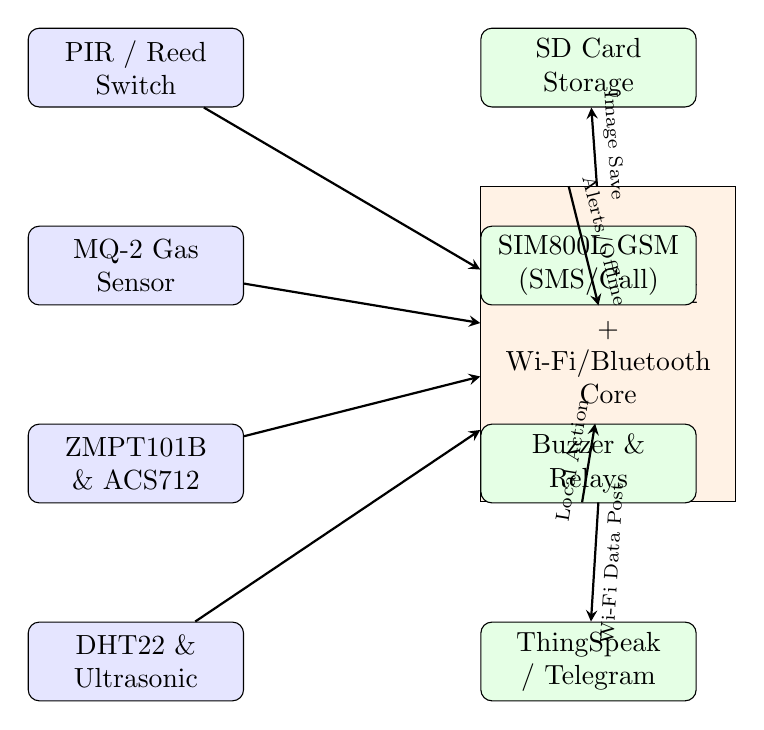
\begin{tikzpicture}[node distance=1.5cm and 2cm]
        
        % Sensors (Left)
        \node (pir) [sensor] {PIR / Reed Switch};
        \node (mq2) [sensor, below=of pir] {MQ-2 Gas Sensor};
        \node (power) [sensor, below=of mq2] {ZMPT101B \& ACS712};
        \node (dht) [sensor, below=of power] {DHT22 \& Ultrasonic};
        
        % MCU (Center)
        \node (mcu) [mcu, right=3cm of mq2, yshift=-1cm] {\textbf{ESP32-CAM} \\ + \\ Wi-Fi/Bluetooth Core};
        
        % Outputs (Right)
        \node (sd) [output, right=3cm of pir] {SD Card Storage};
        \node (gsm) [output, below=of sd] {SIM800L GSM (SMS/Call)};
        \node (relay) [output, below=of gsm] {Buzzer \& Relays};
        \node (cloud) [output, below=of relay] {ThingSpeak / Telegram};
        
        % Arrows
        \draw [arrow] (pir) -- (mcu);
        \draw [arrow] (mq2) -- (mcu);
        \draw [arrow] (power) -- (mcu);
        \draw [arrow] (dht) -- (mcu);
        
        \draw [arrow] (mcu) -- (sd) node[midway, above, sloped, font=\scriptsize] {Image Save};
        \draw [arrow] (mcu) -- (gsm) node[midway, above, sloped, font=\scriptsize] {Alerts/Offline};
        \draw [arrow] (mcu) -- (relay) node[midway, above, sloped, font=\scriptsize] {Local Action};
        \draw [arrow] (mcu) -- (cloud) node[midway, below, sloped, font=\scriptsize] {Wi-Fi Data Post};
        
    \end{tikzpicture}
    \caption{Level 2 Architecture Block Diagram}
    \label{fig:block_diagram}
\end{figure}


\section{Costing Analysis (100 Unit Deployment)}
For a hypothetical mass deployment of 100 units, economies of scale apply. Below is the estimated Bill of Materials (BOM) cost.

\begin{table}[H]
\centering
\begin{tabular}{|l|c|c|c|}
\hline
\textbf{Component} & \textbf{Unit Price (USD)} & \textbf{Qty per Unit} & \textbf{Cost for 100 Units} \\ \hline
ESP32-CAM Module & \$ 5.50 & 1 & \$ 550.00 \\ \hline
SIM800L GSM Module & \$ 3.50 & 1 & \$ 350.00 \\ \hline
ZMPT101B \& ACS712 & \$ 4.00 & 1 set & \$ 400.00 \\ \hline
MQ-2 Gas Sensor & \$ 1.20 & 1 & \$ 120.00 \\ \hline
Environment Sensors (DHT22, etc) & \$ 6.00 & 1 set & \$ 600.00 \\ \hline
Misc (Relays, Buzzers, Reed Switch) & \$ 3.00 & 1 set & \$ 300.00 \\ \hline
Custom PCB, Enclosure \& Power & \$ 10.00 & 1 set & \$ 1,000.00 \\ \hline
\textbf{Total Estimated Cost} & \textbf{\$ 33.20} & \textbf{-} & \textbf{\$ 3,320.00} \\ \hline
\end{tabular}
\caption{BOM Cost Estimation for 100 Units}
\end{table}

\section{Deliverables \& Conclusion}
The completed Level 2 system meets the following deliverables:
\begin{enumerate}
    \item \textbf{Working Prototype:} All 7 sensors, GSM, and ESP32-CAM assembled.
    \item \textbf{Live Dashboard Link:} Telegram bot access and ThingSpeak data stream displaying at least 48 hours of power and environment logs.
    \item \textbf{System Resilience:} Demonstrated ability to fall back to GSM alerts when Wi-Fi is forcefully disconnected.
\end{enumerate}

\textbf{Conclusion:} 
The upgrade to Level 2 successfully transformed a basic localized room monitor into a highly secure, resilient, and intelligent IoT node. By introducing image capture capabilities and out-of-band cellular alerts, the system overcomes the primary weaknesses of standard Wi-Fi dependent smart-home devices. The addition of power monitoring provides critical insights into grid stability and energy footprint, making this an ideal prototype for deployment in environments with unreliable power grids or intermittent internet connectivity.

\end{document}
